\section{Software and Connectivity}

\subsection{BLE Compatibility With the VESC}

\subsubsection{First Experiment}
VESC-controllers are not necessarily equipped with Bluetooth-modules by default. Often, it is necessary to add a BLE-module. A standard HC-05 bluetooth-module compatible with Arduino is a great way to send and receive bluetooth-packets from a host, e.g. a mobile phone, via a bridge translating the bluetooth packets to the UART protocol. This could be demonstrated using a ESP8622's standard library with said module, by letting us send characters from one device to another.

\subsubsection{HC-05 and the VESC}
By flashing the VESC firmware on a discovery-card and connecting the HC-05 module to the PB10 and PB11-pins, which are the Rx and Tx-pins for the STM32F4xx chip, we discovered that the setup for the bluetooth module was not available in the VESC tool. The inherent BLE capabilities is an important limitation to consider when designing a VESC system. We learned therefore that the HC-05 is not originally adapted for BLE. The need for a bridge also adds on complexity and cost, in the form of extra components and another device to maintain the code of. For the future, choosing a bluetooth module supporting BLE will be the easiest solution. Preferably a module fitting the communication connector on the cheap FOCer project \cite{shamansystems_cheap-focer-2firmware_nodate} could facilitate the relevancy of the PCB project with a microcontroller.

\subsubsection{BLE Vulnerability}
Bluetooth could be a vulnerability to a VESC if it is to be used as a controller in real-time, as the controller could be jammed. Our test with the Flipper Zero shows the disfunctionnality of Bluetooth with different use cases. We experienced with the jamming of a bluetooth speaker that the music completely stopped. It could also be investigated how the connection to the VESC could be modified using the VESC tool. We will touch more on the accessibility of the code within the VESC tool sooner.

\subsection{Setup of BT-connection with VESC}
The setup consisted of a main PC/controller, HC-05 Bluetooth module, ESP8266 µ-controller, STM32 Discovery µ-controller, PC with VESC-tool as well as a \textit{FlipperZero}. Our plan of action consisted of flashing the Discovery-card with code for then to read this code via UART to the ESP8266 which was connected to the BT-module. The BT-module would then send packets to the PC. This PC would then act as read/write to read the code having been flashed on the Discovery. Full-band jamming would then be achieved by the implementation of the \textit{FlipperZero} disrupting any transfer of code from PC1 to PC2.The \textit{FlipperZero} was equipped with the firmware \textit{DarkFlippers/unleashed-firmware}\cite{noauthor_darkflippersunleashed-firmware_2026} with the addition of an NRF-jammer from \textit{huuck/FlipperZeroNRFJammer} \cite{cirlig_huuckflipperzeronrfjammer_2026}.

\newpage

\begin{figure}[!h]
    \centering 

\begin{tikzpicture}

% PC_ESP
\node[
    draw,
    rectangle,
    minimum width=1.5cm,
    minimum height=1.5cm
] (PC1) at (2.5,-0.5)
{
   
\includegraphics[width=1.5cm]{Figures/PC_STOCK.jpg}
};
\node[above=2mm of PC1] {PC1 ready to r/w};


% HC05
\node[
    draw,
    rectangle,
    minimum width=1.5cm,
    minimum height=1.5cm
] (HC05) at (-0.3,-2.6)
{
   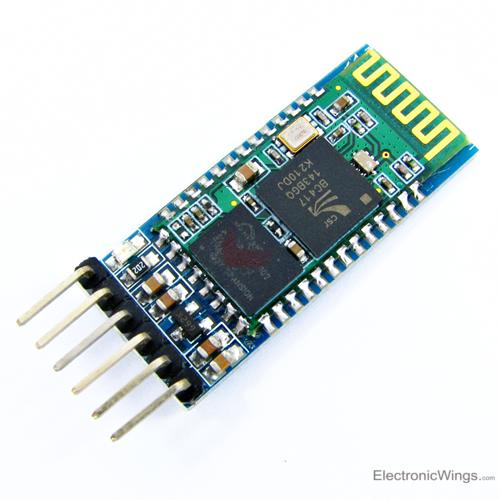
\includegraphics[width=1.5cm]{Figures/HC-05_Bluetooth_Module.jpg}
};
\node[above=1mm of HC05] {HC-05};

\node[
    draw,
    rectangle,
    minimum width=1.5cm,
    minimum height=1.5cm
] (ESP) at (-0.3,-5)
{
    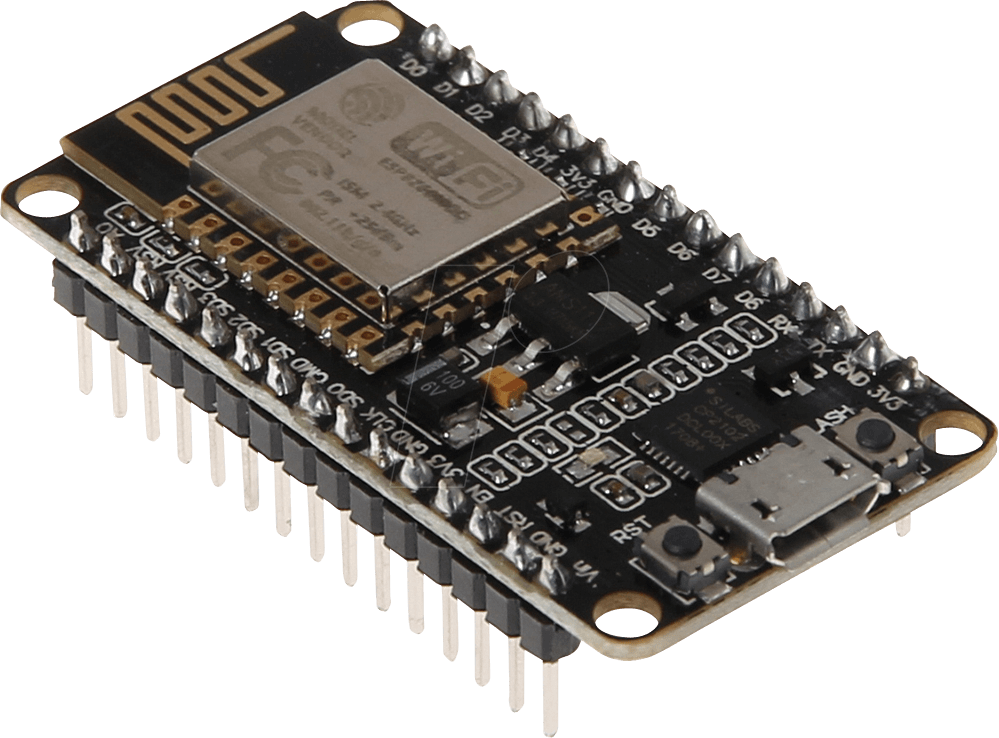
\includegraphics[width=1.5cm]{Figures/ESP8266.png}
};
\node[below=1mm of ESP] {ESP8266};

\node[
    draw,
    rectangle,
    minimum width=1.5cm,
    minimum height=1.5cm
] (PC2) at (-3.6,-2.6)
{
    
\includegraphics[width=1.5cm]{Figures/PC_STOCK.jpg}
};
\node[above=1mm of PC2] {PC2 with VESC-tool};

\node[
    draw,
    rectangle,
    minimum width=1.5cm,
    minimum height=1.5cm
] (Disc) at (-3.6,-5)
{
   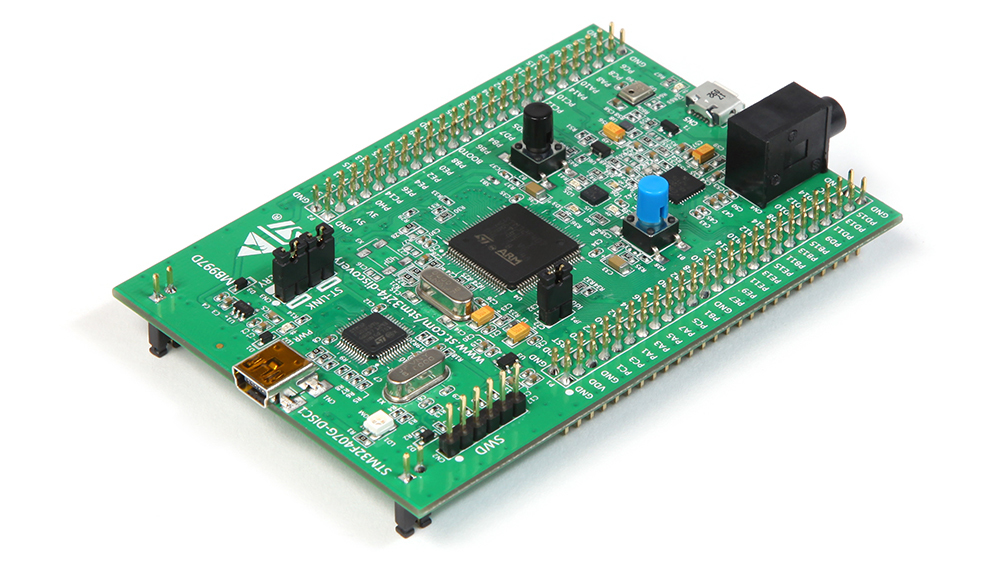
\includegraphics[width=1.5cm]{Figures/STM32_Discovery.jpg}
};
\node[below=1mm of Disc] {STM32 Discovery};

\node[
    draw,
    rectangle,
    minimum width=1.5cm,
    minimum height=1.5cm
] (F0) at (-1.5,0)
{
    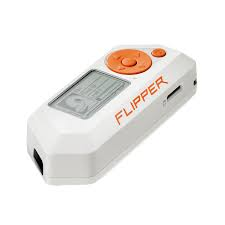
\includegraphics[width=1.5cm]{Figures/F0.jpeg}
};
\node[above=1mm of F0] {FlipperZero};

% Arrow between boxes
%\draw[decorate, decoration={snake}] (box1) -- (box2);
\draw[->, thick] (HC05) -- (ESP);
\draw[<->, decorate, decoration={snake}] (PC1) -- node[below right]{BT-connectivity} (HC05);
\draw[->] (HC05) -- node[left]{UART} (ESP);
\draw[<->] (HC05) -- node[right]{Tx $\leftrightarrow$ Rx} (ESP);

\draw[<->] (ESP) -- node[below]{UART} (Disc);
\draw[<->] (ESP) -- node[above]{Tx $\leftrightarrow$ Rx} (Disc);

\draw[<->] (Disc) -- node[left]{USB} (PC2);

\draw[->, decorate, decoration={snake}] (F0) -- node[above=3mm]{Jamming} (1.25,-1.5);
\

\end{tikzpicture}
 \caption{Setup of BT-connection wih VESC.} 
  \label{fig:BT} 

\end{figure}



\subsection{Code integrity}
\subsubsection{Context}
As the project is open source, and the code is freely accessible, there should be no reason to hide the code. It could however be reasonable to protect the code from changes which could hurt other people. Changing following parameters should at least come with a disclaimer and clearly state the dangers possible by proceeding with said changes. We have in mind the maximum speed permitted and the power available to the motors.

\subsubsection{LispBM extraction}
We caught word that the lisp code for the VESC used by Maillon mobility was easy to extract. By building an older firmware with the Maillon mobility software, we observed this by going to the lispBM tab and clicking read. It's up to the MAD if they would like to reinforce this mechanism. A modification on a parameter and then clicking upload allowed us to easily change the speed limit. This could bring up a public danger. This raises questions on the use of the MAD's equipment, as it's used in a day-to-day traffic environment. 

\subsubsection{LispBM Code}
When we flashed newer firmware from the project made by Benjamin Vedder\cite{b1}, we also observed some difficulties in uploading the lispBM script taken from the one on firmware version 6.06. This could indicate that there needs to be further maintenance of the code in order to get the software up to date. This needs to be documented better for someone  to continue the project. This could be a good investment for the MAD.

This documentation could be as simple as referencing the relevant parts of the lispBM documentation. \cite{b2}

\subsubsection{Proposed Solution}
This risk could be patched by developing a VESC application for the VESC controller or using a binary. This is a solution which is less open source, but defends well against malicious intent.The application could be created using C and use an algorithm known by the MAD in order to secure the access to someone to change the parameters only if they are MAD certified personnel. This encryption would preferably be reduced to the most essential settings in order to align with what our impression of the philosophy of the MAD would be.


\subsection{VESC Compiling}
As mentioned, we have been able to compile the VESC tool and the VESC firmware. This firmware has been put onto an STM32F4xx Discovery card. This card uses the same chip as the aforementioned ``Cheap FOCer'' project. The thought was that using something with the same chip would facilitate the switch from the discovery card to a PCB with the same target.

However, this choice posed several obstacles for our progress on the topic of cybersecurity. We will nonetheless summarise what we have learned for you and propose some additional work for the future. The challenges we encountered were the following: The lack of bluetooth capabilities. We did not have a module with BLE either. We had access to a HC-05 module, but that only allows for a normal Bluetooth version 2.0 protocol and would require further work on a bridge to UART by using an esp8622 that we had as well. We propose that the next group has access to a VESC controller from the beginning, as well as a motor we could control. This could be in cooperation with the MAD, as the MAD could propose some models they're interested in.

We also found that the information on the VESC is scattered around the internet. The resources is also sometimes based on a Debian-based Linux system which adds more work for someone using another distribution of Linux. This could hinder the implementation facility for new users. We struggled particularly with the Qt packages for positioning and game pad. We would therefore recommend the use of a Debian-based Linux system for the computer working with the VESC for the MAD associates.




